\documentclass[e4_tp1_main.tex]{subfiles}

\begin{document}

\section{Ejercicio 3}



\begin{landscape}
	\vspace*{\fill}
	\begin{figure}[ht]
		\centering
		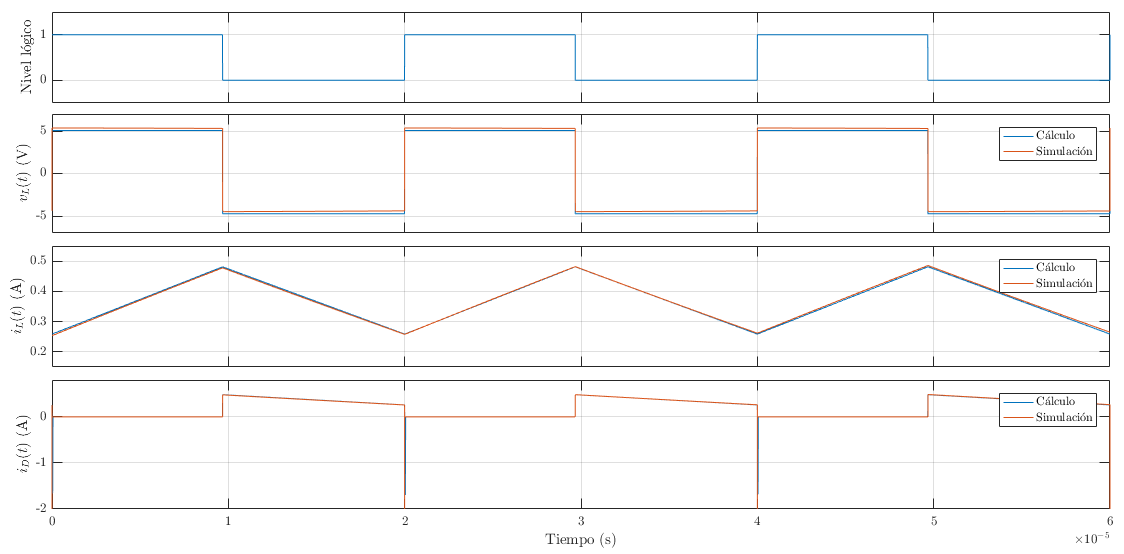
\includegraphics[scale=0.75]{images/ej2/curvas.png}
		\caption{Curvas te\'oricas y simuladas de la fuente buck: de arriba hacia abajo, estado de la llave (abierta en 0), tensi\'on en la bobina, corriente en la bobina, y corriente en el diodo.}
		\label{fig:buck-curvas}
	\end{figure}
	\vspace*{\fill}
\end{landscape}


\end{document}